%%%%%%%%%%%%%%%%%%%%%%%%%%%%%%%%%%%%%%%%%
% Jacobs Landscape Poster
% LaTeX Template
% Version 1.1 (14/06/14)
%
% Created by:
% Computational Physics and Biophysics Group, Jacobs University
% https://teamwork.jacobs-university.de:8443/confluence/display/CoPandBiG/LaTeX+Poster
% 
% Further modified by:
% Nathaniel Johnston (nathaniel@njohnston.ca)
%
% This template has been downloaded from:
% http://www.LaTeXTemplates.com
%
% License:
% CC BY-NC-SA 3.0 (http://creativecommons.org/licenses/by-nc-sa/3.0/)
%
%%%%%%%%%%%%%%%%%%%%%%%%%%%%%%%%%%%%%%%%%

%----------------------------------------------------------------------------------------
%	PACKAGES AND OTHER DOCUMENT CONFIGURATIONS
%----------------------------------------------------------------------------------------

\documentclass[final,a0,portrait]{beamer}

\usepackage[scale=1.17]{beamerposter} % Use the beamerposter package for laying out the poster

\usetheme{confposter} % Use the confposter theme supplied with this template

\setbeamercolor{block title}{fg=ngreen,bg=white} % Colors of the block titles
\setbeamercolor{block body}{fg=black,bg=white} % Colors of the body of blocks
\setbeamercolor{block alerted title}{fg=white,bg=dblue!70} % Colors of the highlighted block titles
\setbeamercolor{block alerted body}{fg=black,bg=dblue!10} % Colors of the body of highlighted blocks
% Many more colors are available for use in beamerthemeconfposter.sty

%-----------------------------------------------------------
% Define the column widths and overall poster size
% To set effective sepwid, onecolwid and twocolwid values, first choose how many columns you want and how much separation you want between columns
% In this template, the separation width chosen is 0.024 of the paper width and a 4-column layout
% onecolwid should therefore be (1-(# of columns+1)*sepwid)/# of columns e.g. (1-(4+1)*0.024)/4 = 0.22
% Set twocolwid to be (2*onecolwid)+sepwid = 0.464
% Set threecolwid to be (3*onecolwid)+2*sepwid = 0.708

\newlength{\sepwid}
\newlength{\onecolwid}
\newlength{\twocolwid}
\newlength{\threecolwid}
%\setlength{\paperwidth}{48in} % A0 width: 46.8in
%\setlength{\paperheight}{36in} % A0 height: 33.1in
\setlength{\paperwidth}{86.1cm} % A0 width: 46.8in
\setlength{\paperheight}{118.9cm} % A0 height: 33.1in
\setlength{\sepwid}{0.01\paperwidth} % Separation width (white space) between columns
\setlength{\onecolwid}{0.3013\paperwidth} % Width of one column
\setlength{\twocolwid}{0.6026\paperwidth} % Width of two columns
\setlength{\threecolwid}{0.9040\paperwidth} % Width of three columns
\setlength{\topmargin}{-0.5in} % Reduce the top margin size
%-----------------------------------------------------------

\usepackage{tikz}
\usetikzlibrary{mindmap, backgrounds, calc}
\definecolor{Gold}{rgb}{0.64,0.54,0.29}

\usepackage{graphicx}  % Required for including images
\graphicspath{{figures/}} % Directory in which figures are stored

\usepackage{booktabs} % Top and bottom rules for tables

\usepackage{multicol}
%-----------------------------------------------------------------------------
%	TITLE SECTION 
%----------------------------------------------------------------------------

\title{Assessing GNSS-derived displacements at the near and far-field of the 2023 Turkey earthquake doublet} % Poster title
% \subtitle{}

\author{Panagiotis Psimoulis\textsuperscript{a}, \underline{Dimitrios Anastasiou}\textsuperscript{b}, Xanthos Papanikolaou\textsuperscript{b}, Maria Tsakiri\textsuperscript{b}}% Author(s)

%\institute{Dionysos Satellite Observatory, School of Rural, Surveying \& Geoinformatics Engineering \\ \vspace{0.5em} \par{National Technical University of Athens}} % Institution(s)
\institute{\textsuperscript{a} Faculty of Engineering,  University of Nottigham \\
\textsuperscript{b} School of Rural, Surveying \& Geoinformatics Engineering, National Technical University of Athens} % Institution(s)

%----------------------------------------------------------------------------------------

\begin{document}

\addtobeamertemplate{block end}{}{\vspace*{2ex}} % White space under blocks
\addtobeamertemplate{block alerted end}{}{\vspace*{2ex}} % White space under highlighted (alert) blocks

\setlength{\belowcaptionskip}{2ex} % White space under figures
\setlength\belowdisplayshortskip{2ex} % White space under equations

\begin{frame}[t] % The whole poster is enclosed in one beamer frame

\begin{columns}[t] % The whole poster consists of three major columns, the second of which is split into two columns twice - the [t] option aligns each column's content to the top

\begin{column}{\sepwid}\end{column} % Empty spacer column

\begin{column}{\onecolwid} % The first column

%----------------------------------------------------------------------------------------
%	INTRODUCTION
%----------------------------------------------------------------------------------------

\begin{block}{Introduction}
{\small

}
\vspace*{20cm}
test
\end{block}

%------------------------------------------------
%    SOFTWARE DESING
%------------------------------------------------
\begin{block}{Network \& Data processing}
{\small
57 continuously operating GNSS stations in distances ranging from 900km to 1400km from the epicenter
Receiver type: LEICA

- most of them GR30

- also GRX1200GGPRO / GRX1200+GNSS

Antenna type LEICA

- LEIAR10 / LEIAS10

- few stations: LEIAX1202GG

Observation interval: 1s

Precise Point Positioning w Ambiguity Resolution

Sat systems:

GPS / GLO / GAL / BDS-2/3

Elevation angle: 7 deg

--Kinematic mode

Reference Frame: IGS20

Final IGS Products for satellite:

- Orbits (.SP3)

- Clocks (.CLK)

- Earth Orientation Parameters (.ERP)

- Attitude (.OBX)

- Bias (.BIA)

ANTEX File: IGS20\_2247

For Tropospheric modeling: VMF1
}
%\begin{center}
%  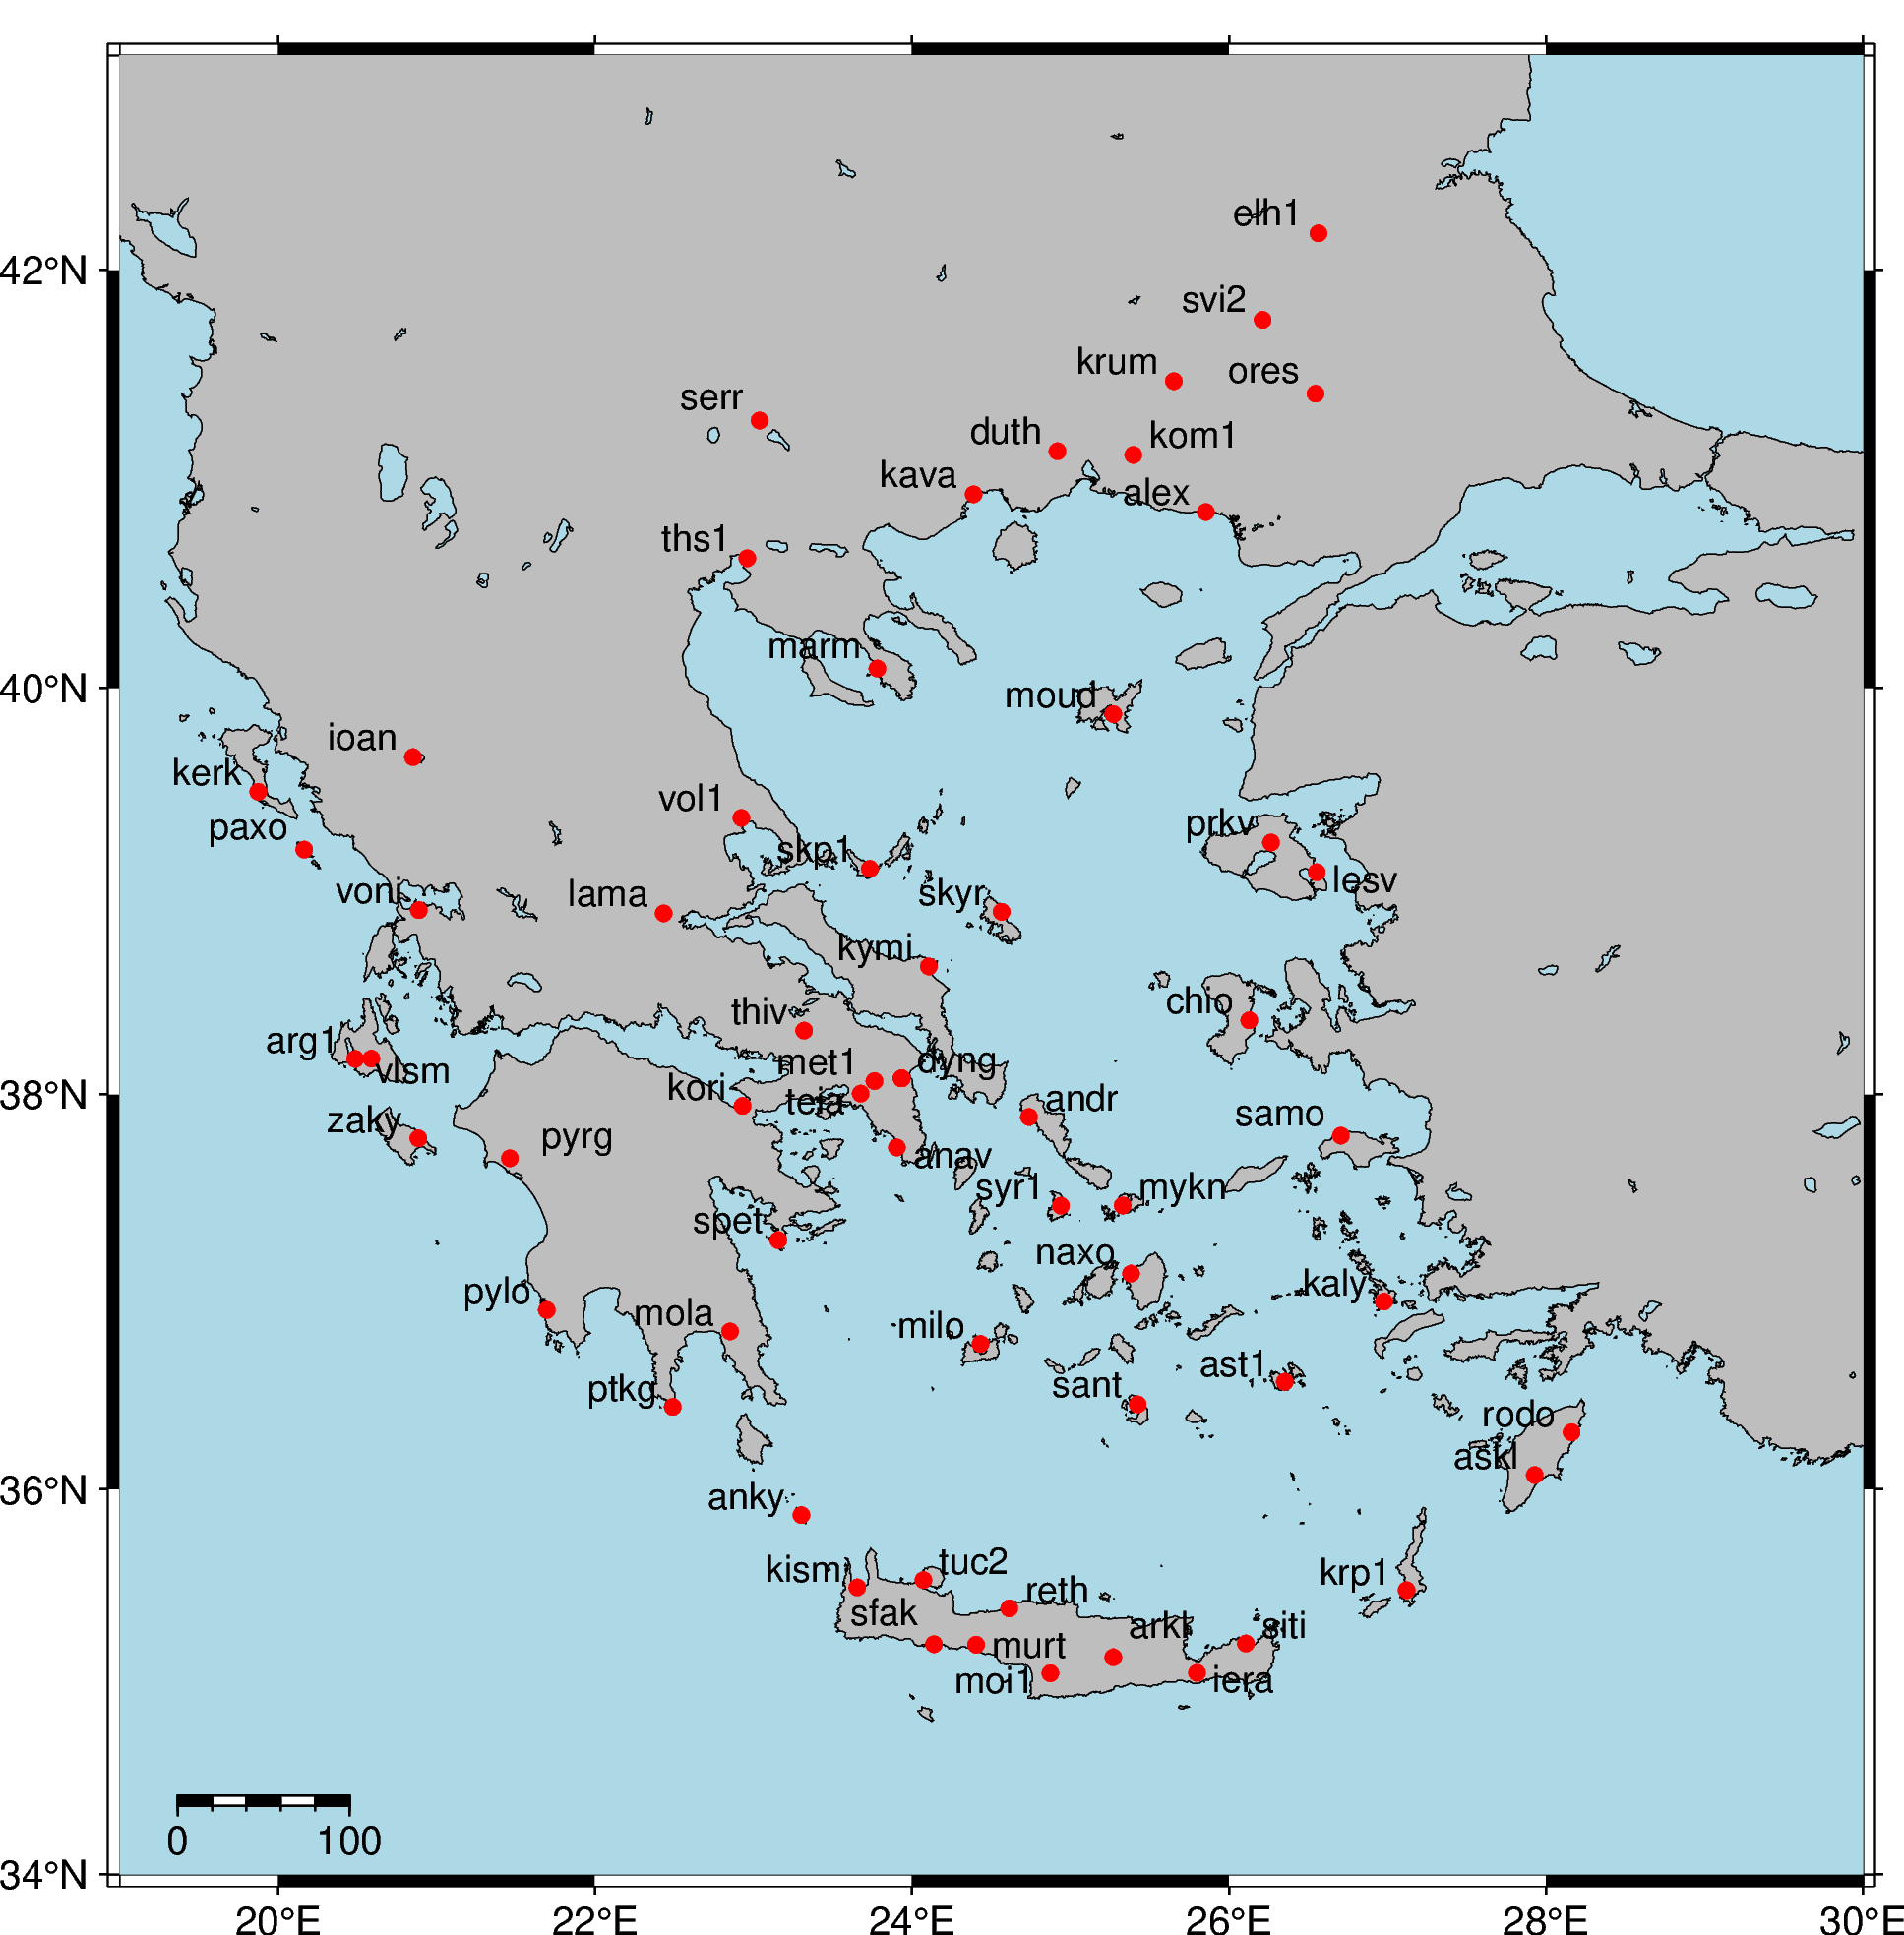
\includegraphics[width=.97\textwidth]{figures/gnss_network.png}
%\end{center}
%\vspace*{48cm}
\end{block}
\begin{figure}
\begin{center}
  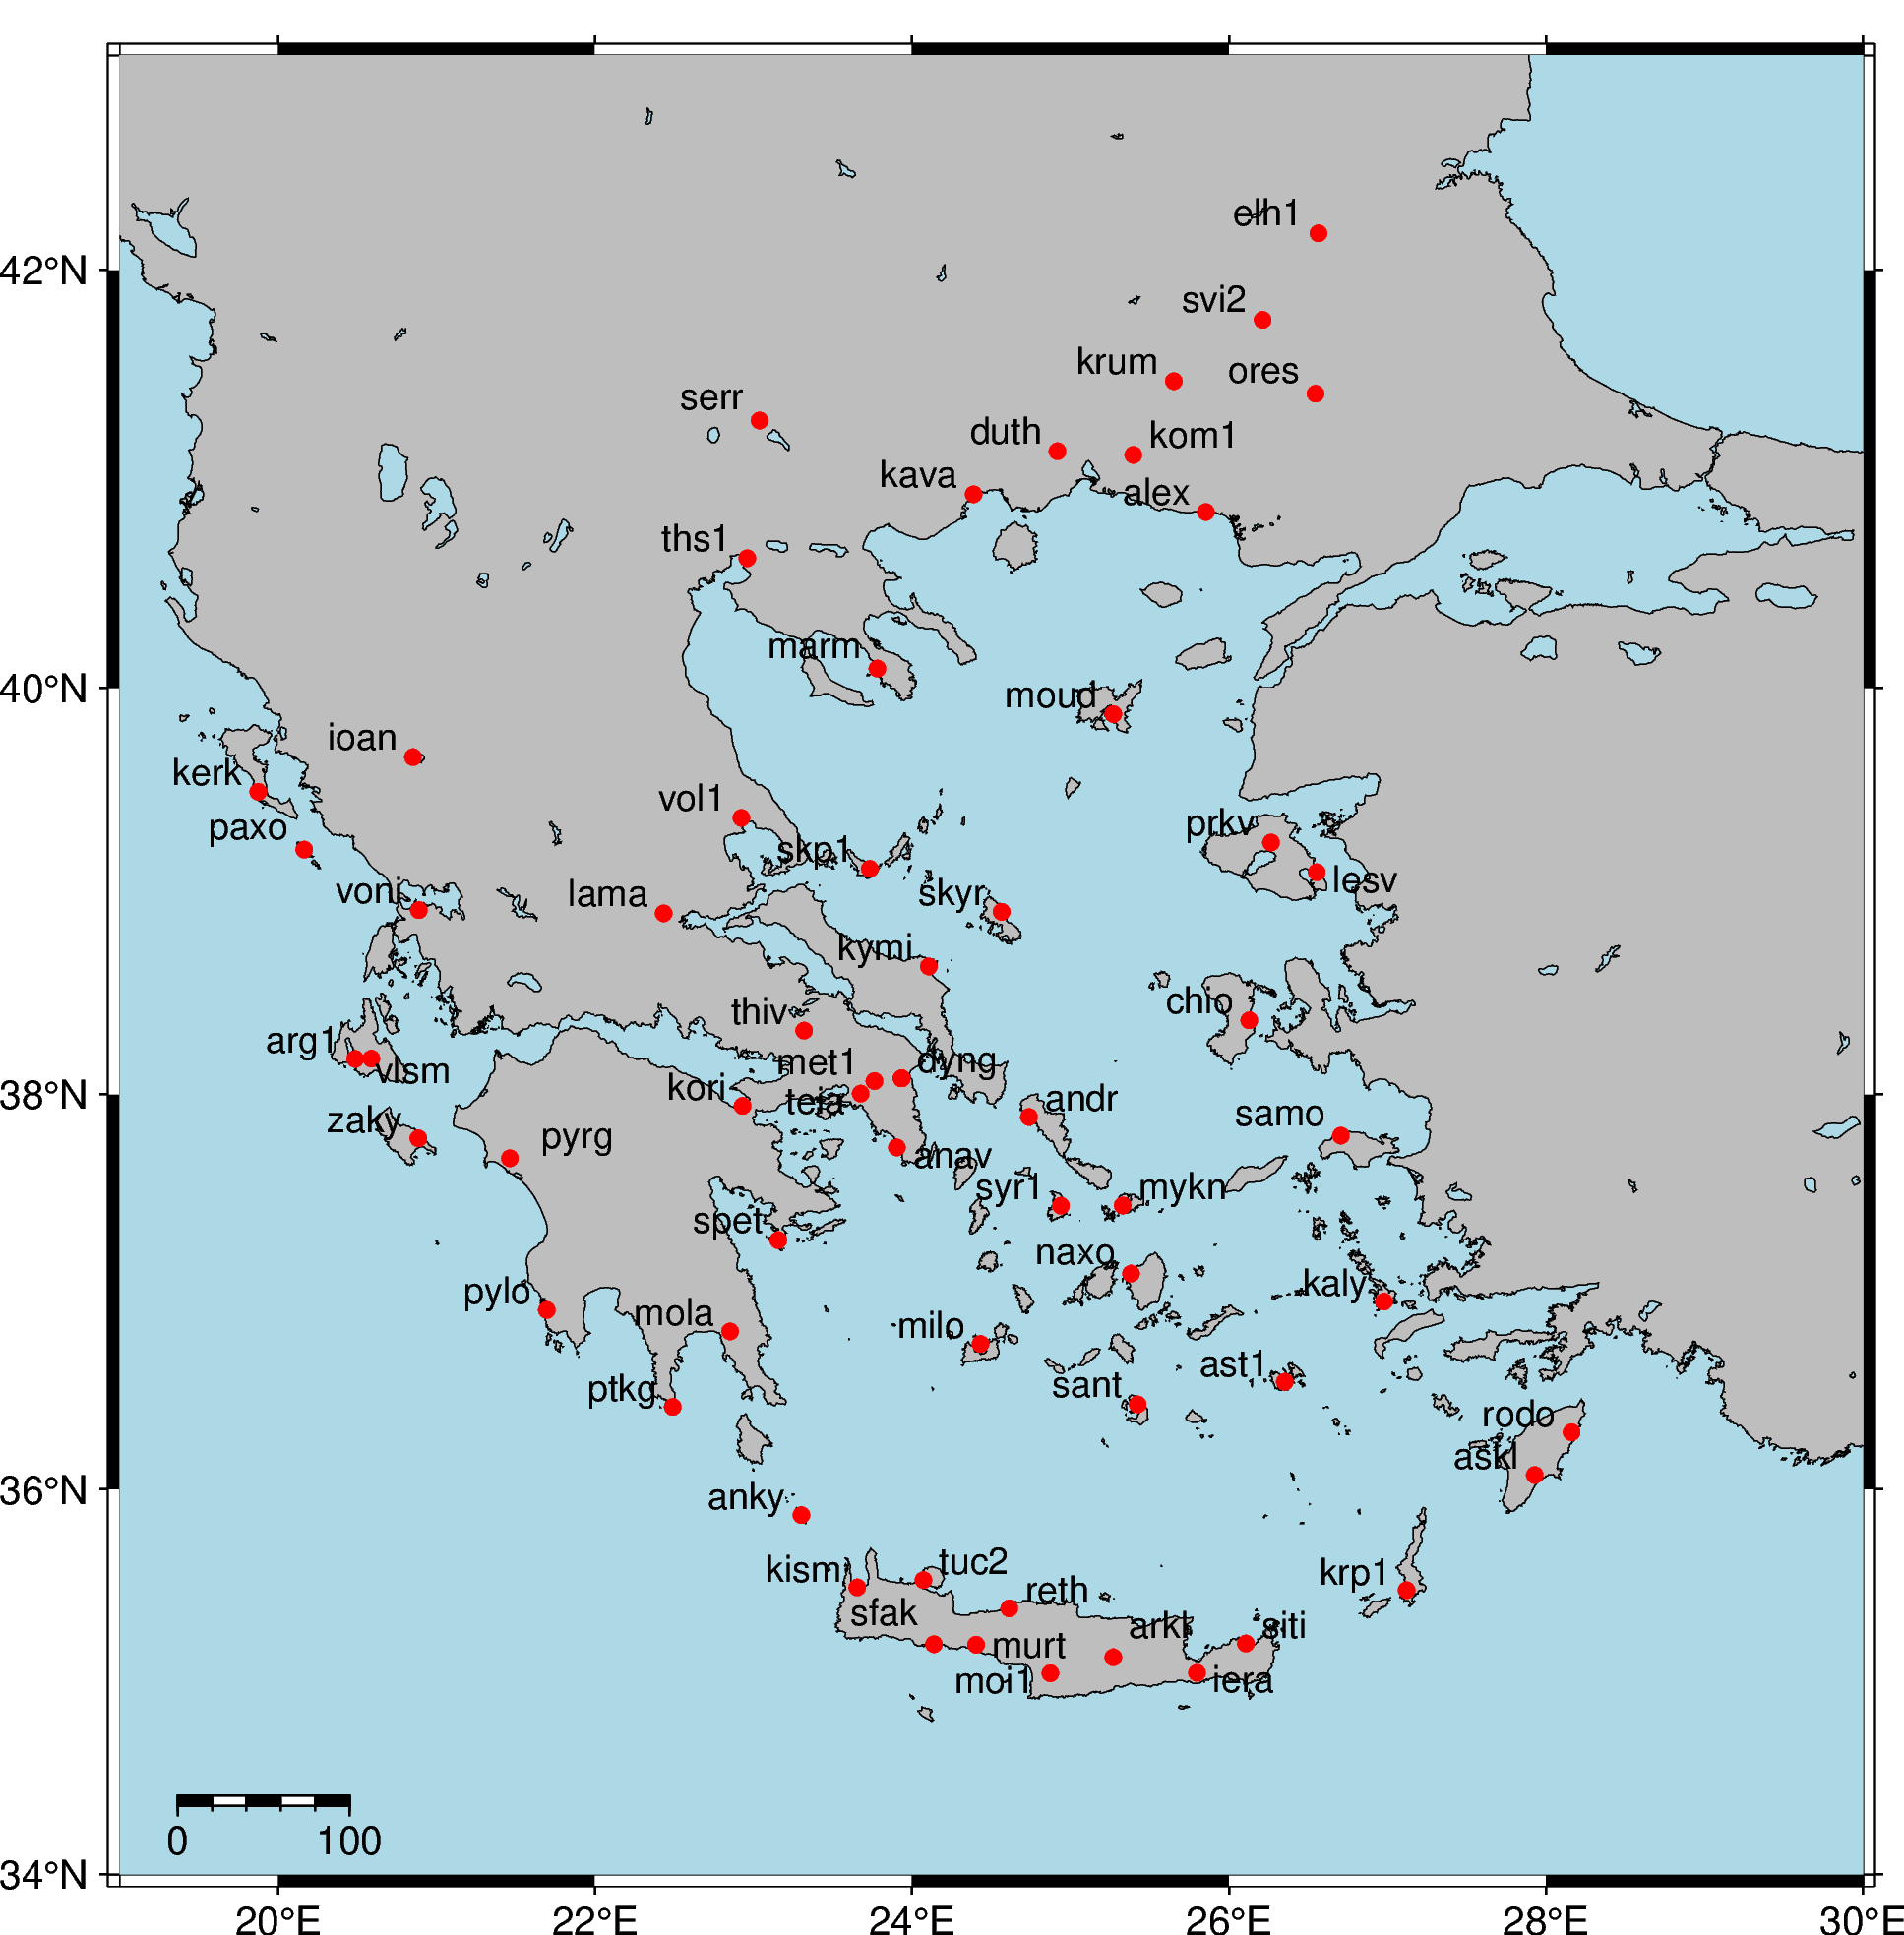
\includegraphics[width=.97\textwidth]{figures/gnss_network.png}
\end{center}
    \caption{Processed stations.}
    \label{fig:proc-net}
\end{figure}      

%\bigskip
%\begin{alertblock}{Contact Information}
%\begin{itemize}
%\item Web: \href{http://dionysos.survey.ntua.gr}{dionysos.survey.ntua.gr}
%\item Email: \href{xanthos@mail.ntua.gr}{xanthos@mail.ntua.gr}
%\end{itemize}
%\end{alertblock}
\vfill
%----------------------------------------------------------------------------
%	CONTACT INFORMATION
%----------------------------------------------------------------------------
%\setbeamercolor{block alerted title}{fg=black,bg=norange} % Change the alert block title colors
%\setbeamercolor{block alerted body}{fg=black,bg=white} % Change the alert block body colors
\begin{minipage}{\twocolwid}
\vspace*{1.0\baselineskip}
\begin{center}
  
\includegraphics[width=.97\textwidth]{figures/ESC2024_webheader.png}
\end{center}
\end{minipage}
%
%\begin{alertblock}{Contact Information}
%\begin{itemize}
%\item Web: \href{http://dionysos.survey.ntua.gr}{dionysos.survey.ntua.gr}
%\item Email: \href{xanthos@mail.ntua.gr}{xanthos@mail.ntua.gr}
%\end{itemize}
%\end{alertblock}



%-----------------------------------------------------------------------------

\end{column} % End of the first column
%\vrule{}

% Empty spacer column
\begin{column}{\sepwid}\end{column}

% Begin a column which is two columns wide (column 2)
\begin{column}{\onecolwid} 

%--------------------------------------------------------------------------
%	PROCESSING
%---------------------------------------------------------------------------

\begin{block}{Processing \& Analysis}

{\small
TEST
}

%\begin{figure}
%  \centering
%  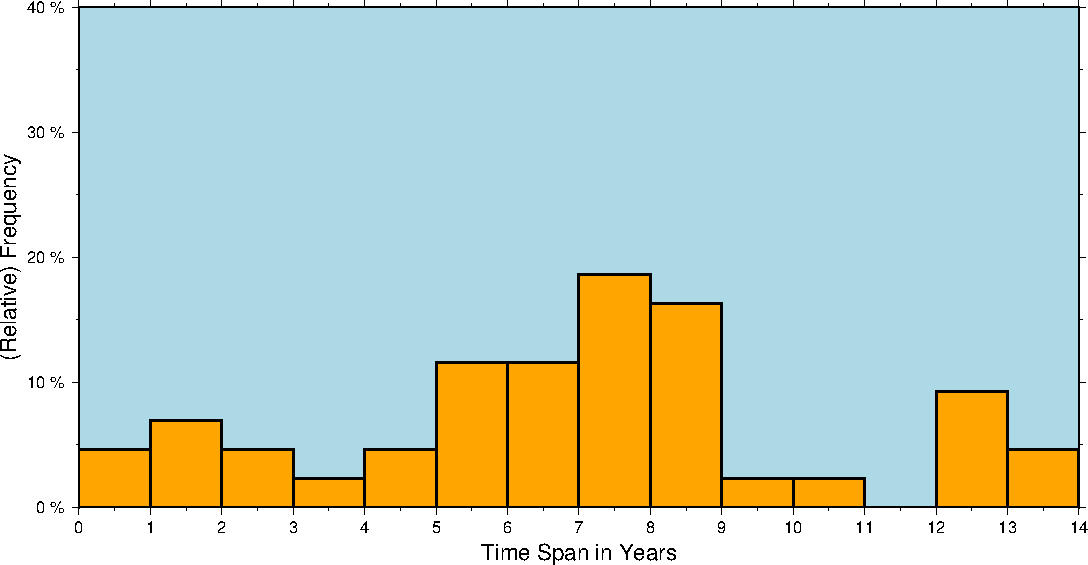
\includegraphics[width=0.7\onecolwid]{sample}
%  \caption{Flowchart of processing work.}
%  \label{fig:proc}
%\end{figure}
\end{block}

%-------------------------------------------------------------------------
%	PRELIMINARY RESULTS
%-------------------------------------------------------------------------
%\begin{block}{Preliminary Results}
%{\small
%\end{block}
%-----------------------------------------------------------------------------

\end{column} % End of the second column

\begin{column}{\sepwid}\end{column} % Empty spacer column

%\vrule{}

\begin{column}{\onecolwid} % The third column

%----------------------------------------------------------------------------------------
%	ONLINE PLATFORM
%----------------------------------------------------------------------------------------

\begin{block}{}
{\small
}



\end{block}

%---------------------------------------------------------------------------
%	CONCLUSION
%---------------------------------------------------------------------------
\begin{block}{Current Status \& Future Work}
{\small
Currently 

}
\end{block}

%----------------------------------------------------------------------------------------
%	REFERENCES
%----------------------------------------------------------------------------------------

\begin{block}{References}

\nocite{*} % Insert publications even if they are not cited in the poster
\footnotesize{\bibliographystyle{unsrt}
\bibliography{sample}\vspace{0.75in}}


\end{block}

%----------------------------------------------------------------------------------------
%	CONTACT INFORMATION
%----------------------------------------------------------------------------------------

%\setbeamercolor{block alerted title}{fg=black,bg=norange} % Change the alert block title colors
%\setbeamercolor{block alerted body}{fg=black,bg=white} % Change the alert block body colors

\begin{alertblock}{Contact Information}
\begin{itemize}
\item Web: \href{http://dionysos.survey.ntua.gr}{dionysos.survey.ntua.gr}
\item Email: \href{danastasiou@mail.ntua.gr}{danastasiou@mail.ntua.gr}
\end{itemize}
\end{alertblock}
%
%\begin{figure}
%
\includegraphics[width=1.0\linewidth]{ESPA-EKT-GSRT_Logo-EN.JPG}
%\end{figure}                                                            

%----------------------------------------------------------------------------------------

\end{column} % End of the third column

\end{columns} % End of all the columns in the poster

\end{frame} % End of the enclosing frame

\end{document}
